% #############################################################################
% This is Chapter 5
% !TEX root = ../main.tex
% #############################################################################
% Change the Name of the Chapter i the following line
\fancychapter{Results}
\cleardoublepage
% The following line allows to ref this chapter
\label{chap:results}

\par The following results are based on solving the optimisation problem \eqref{eq:multi_cost_bern} with the implementation described in section \ref{sec:description_implementation}.
\par Sequential Quadratic Programming \cite{10.1007/978-0-387-35514-6_7} will be the nonlinear programming solver of choice. Simulations were run on a 4 × Intel\textsuperscript{\textcopyright} Core\texttrademark i5-7200U CPU @ 2.50GHz processor. 


\par Several different running cost functions were tested such as 
\begin{equation}
    J = \int_0^T \frac{du}{dt}^2 dt
\end{equation}
which minimizes tangent acceleration,
\begin{equation}
    J = \int_0^T u^2 dt
\end{equation}
which minimizes speed, and finally, for the Medusa model, specifically,
\begin{equation}
    J = \int_0^T \tau_u^2 + \tau_r^2
\end{equation}
which minimizes the input.
\par All of these serve as proxies to the minimisation of spent energy.

\par Results for the two models presented in chapter \ref{chap:autonomousvehiclemodels} are presented. The unicycle model has a total of 5 state variables while the Medusa model has a total of 6 state variables plus 2 inputs. Upper and lower bounds for each variable for each vehicle were implemented as explained in section \ref{sec:dynamics}, by finding the biggest and smallest control points. For the examples presented in this chapter, the bounds that were used are those presented in table \ref{tab:variablebounds} which were chosen to closer represent a real Medusa vehicle.
\begin{table}[h!]
\centering
\begin{tabular}{|l|l|l|l|}
\hline
& Variable & Starting Conditions & Final Conditions \\ \hline
Dubin's Car & $x$ & $-\infty$ & $\infty$ \\
& $y$ & $-\infty$ & $\infty$ \\
& $\psi$ & $-\infty$ & $\infty$ \\
& $u$ & 0 & 1.1 \\
& $r$ & $-\pi/4$ & $\pi/4$ \\ \hline
Medusa & $x$ & $-\infty$ & $\infty$ \\
& $y$ & $-\infty$ & $\infty$ \\
& $\psi$ & $-\infty$ & $\infty$ \\
& $u$ & 0 & 1.1 \\
& $v$ & $-\infty$ & $\infty$ \\
& $r$ & $-.74$ & $.74$ \\
& $\tau_u$ & 0 & 25.9 \\
& $\tau_r$ & -.113 & .113 \\
\hline
\end{tabular}
\caption{Upper and lower bounds for each variable of each vehicle model}
\label{tab:variablebounds}
\end{table}

\par A significant number of experiments were performed to the optimisation algorithm in order to study its behaviour with changing parameters. Out of all of the experiments that were performed, the most relevant will be presented.

\section{No obstacles}

\par The first problem will be run for both a single Dubin's car and a single Medusa vehicle, with initial and final states described in table \ref{tab:firstproblem} and no obstacles. Figures \ref{fig:noobstaclesfigures} and \ref{fig:noobstaclesmedusa} show solutions for order 20 and a time horizon of . Each example has a different combination of vehicle model and cost function. Both models contain control points to describe $x$ and $y$ positions, which is what the blue lines show. The red lines describe the solution of the Initial Value Problem as described in section \ref{sec:ivproblem}. This figure, and all that remain, flip x and y axis which standard for marine vehicles.

\begin{table}[h!]
\centering
\begin{tabular}{|l|l|l|}
\hline
Variable & Starting Conditions & Final Conditions \\ \hline
$x$ & 0 & 30 \\
$y$ & 0 & 30 \\
$\psi$ & 0 & $\pi/2$ \\
$u$ & 1 & 1 \\
$v$ & 0 & 0 \\
$\omega$ & 0 & 0 \\
\hline
\end{tabular}
\caption{Initial and final conditions for a basic Motion Problem}
\label{tab:firstproblem}
\end{table}


\begin{figure}[h!]
\centering
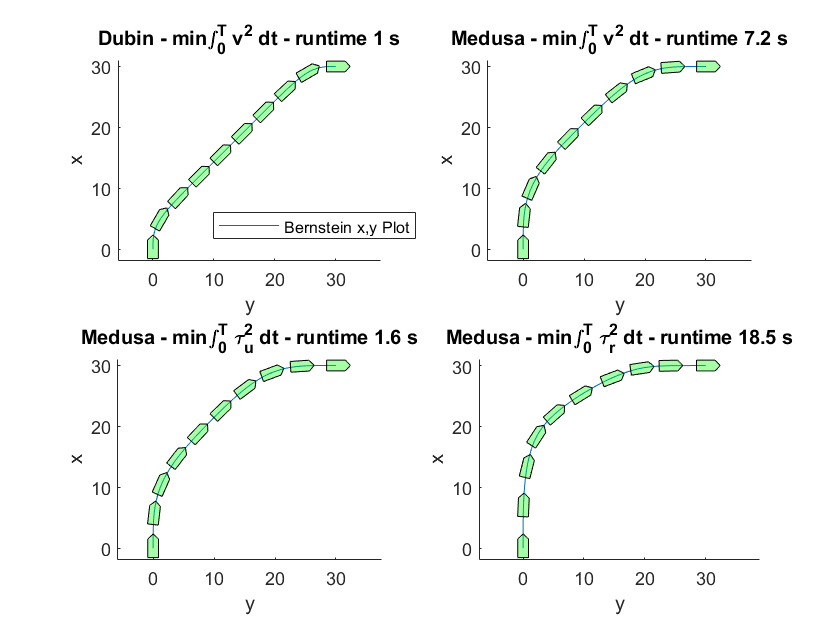
\includegraphics[width=0.8\textwidth]{Images/results/noostaclesfigures.png}
\caption{Solutions of order $N=20$ without obstacles and final time $T=60$}
\label{fig:noobstaclesfigures}
\end{figure}

\begin{figure}[h!]
\centering
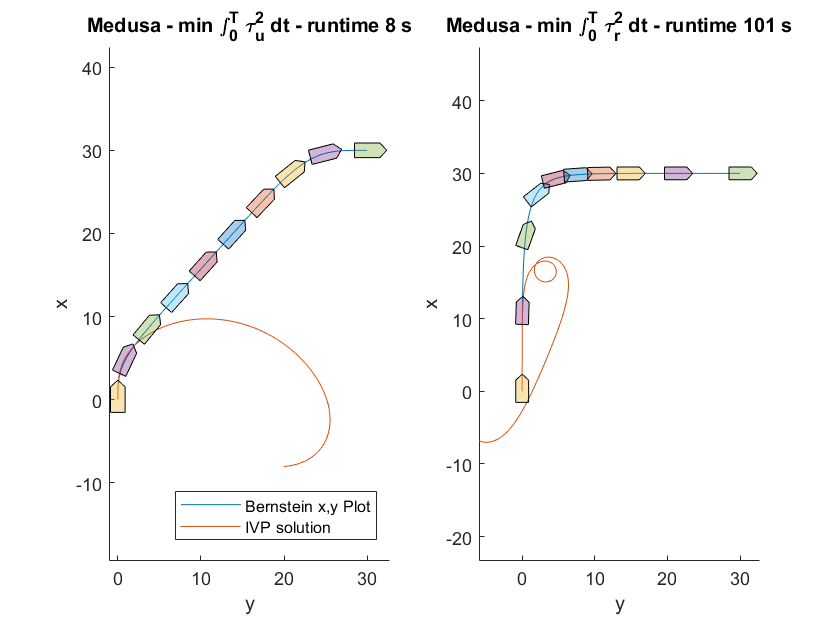
\includegraphics[width=0.8\textwidth]{Images/results/noostaclesmedusa.png}
\caption{Solutions of order $N=20$ that minimize $\tau_u^2$ (left) and $\tau_r^2$ (right) for the Medusa Model with time horizon $T=60$}
\label{fig:noobstaclesmedusa}
\end{figure}

\par First thing to note is, despite all executions running successfully, i. e., the optimal and feasible solution was found, the Medusa's \ac{IVP} solution resembles less the plot of the Bezier curve of the x and y control points when compared with the Dubin's car. This suggests that the order isn't high enough for the curves to accurately represent the real optimal solution's state variables for the Medusa model, which is more complex. 


\section{Obstacles}

\par The following figures show solutions with circle or polygon obstacles whose collision avoidance algorithms are explained in sections \ref{sec:mindistintveh} and \ref{sec:mindistconvshapes}. Figure \ref{fig:baselineresult} is the baseline example without obstacles. It uses a Dubin's Car with the same initial and final conditions as in the previous section and minimises $v^2$. Figure \ref{fig:circleobstacle}, shows the solution with the added circle as a constraint. Figure \ref{fig:circleobstaclelogbargood} shows the solution with an obstacle but the constraint was moved to the log barrier functional as explained in section \ref{sec:logbarrierfunc}. Figure \ref{fig:circleobstaclelogbarbad} shows the solution with log barrier funcitonal as well but the relative weight of the log barrier on the cost wasn't as big, and, as a result, the optimisation problem terminated successfully but did not prevent collision. The runtimes of these examples don't show how the usage of log barrier provides an advantage, however, for a polygon obstacle, such as in figures \ref{fig:polygonobstacle} and \ref{fig:polygonobstaclelogbar} show a huge difference in the usage of the log barrier functional. Both these results have a huge runtime when compared to circular obstacles because the algorithm is iterative.

\begin{figure}[h!]
\centering
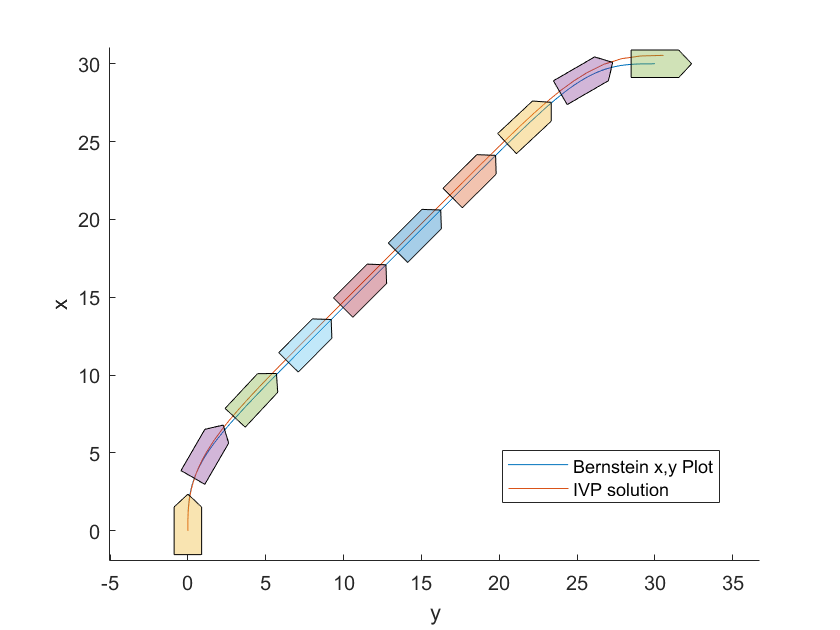
\includegraphics[width=0.8\textwidth]{Images/results/baselineresult.png}
\caption{Solution of order $N=20$ without obstacles \\ computation time = 2s}
\label{fig:baselineresult}
\end{figure}

\begin{figure}[h!]
\centering
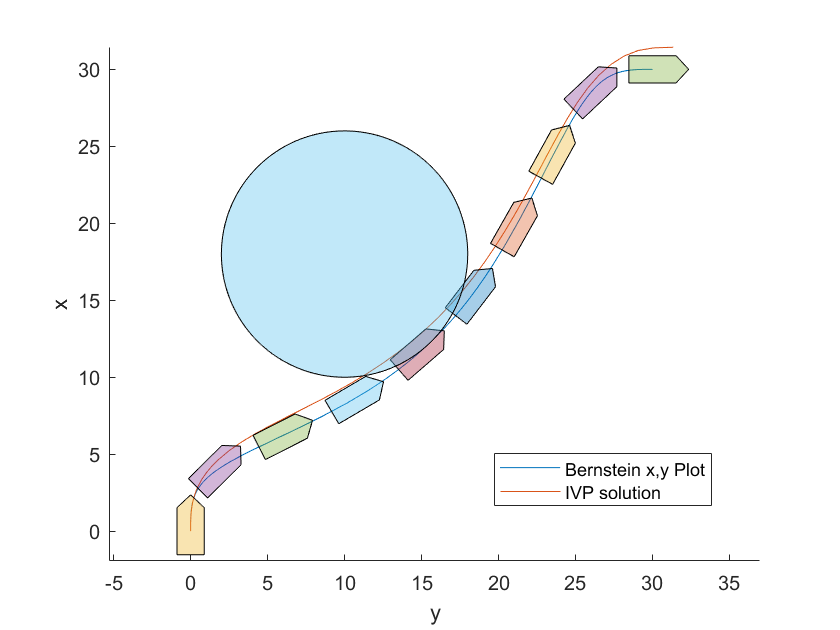
\includegraphics[width=0.8\textwidth]{Images/results/circleobstacle.png}
\caption{Circle osbtacle: computation time 5s}
\label{fig:circleobstacle}
\end{figure}

\begin{figure}[h!]
\centering
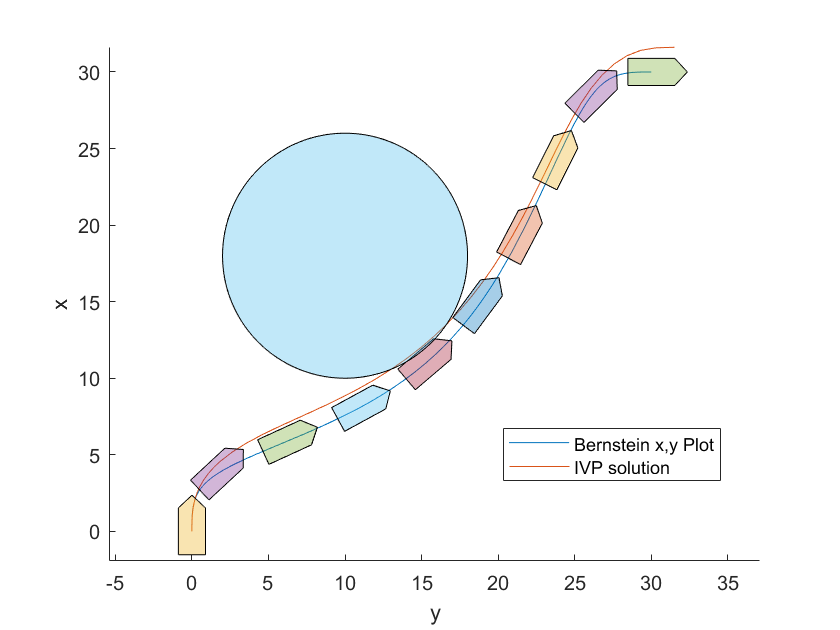
\includegraphics[width=0.8\textwidth]{Images/results/circleobstaclelogbargood.png}
\caption{Circle obstacle plus log bar: computation time 4s}
\label{fig:circleobstaclelogbargood}
\end{figure}

\begin{figure}[h!]
\centering
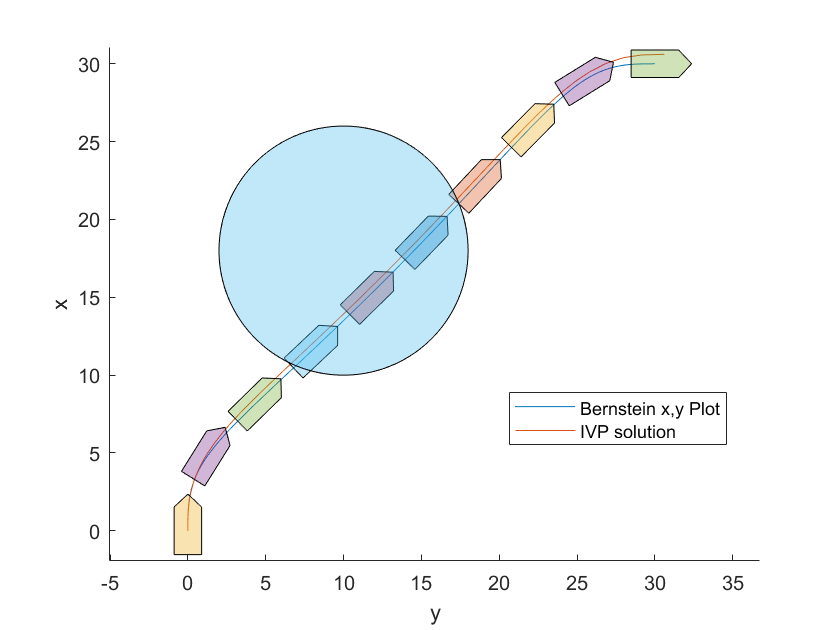
\includegraphics[width=0.8\textwidth]{Images/results/circleobstaclelogbarbad.png}
\caption{Circle obstacle plus log bar: computation time 3s}
\label{fig:circleobstaclelogbarbad}
\end{figure}

\begin{figure}[h!]
\centering
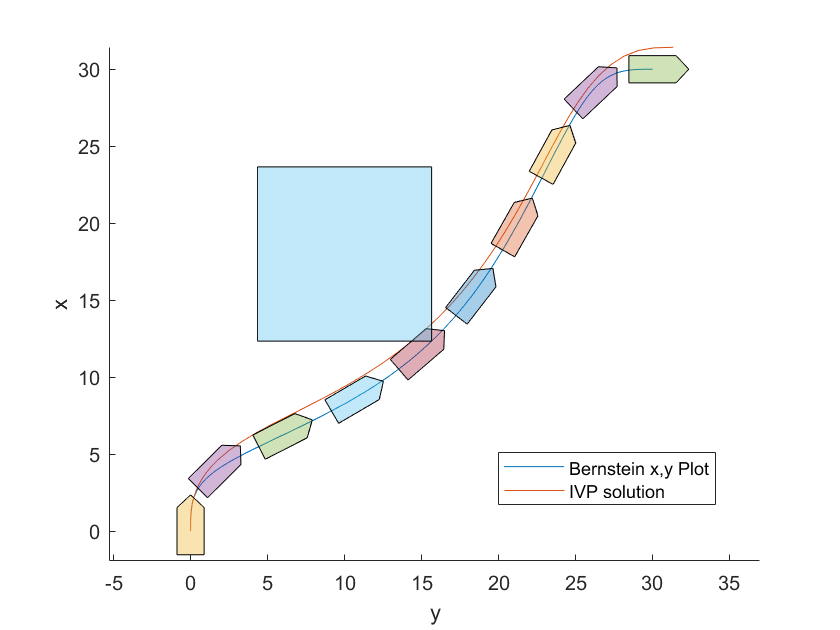
\includegraphics[width=0.8\textwidth]{Images/results/polygonobstacle.png}
\caption{polygon obstacle: computation time 307s}
\label{fig:polygonobstacle}
\end{figure}

\begin{figure}[h!]
\centering
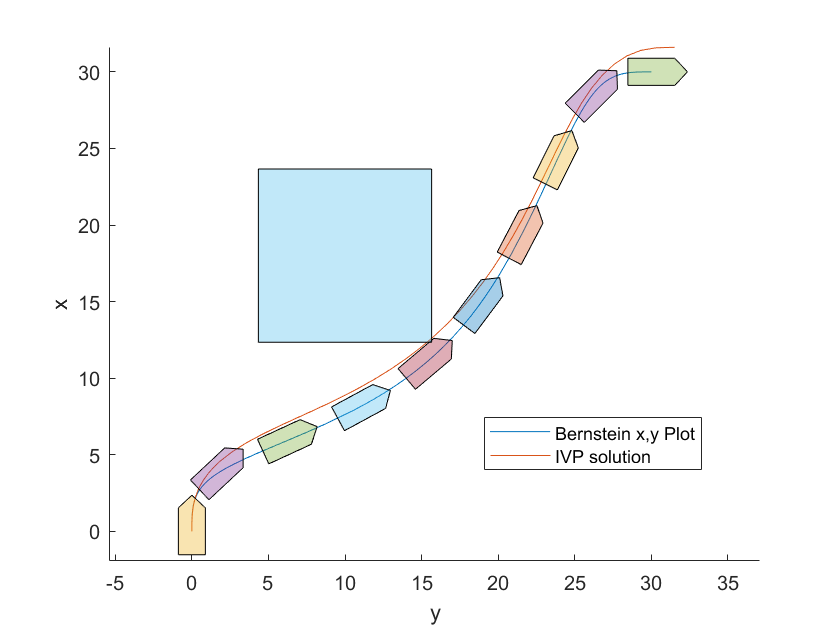
\includegraphics[width=0.8\textwidth]{Images/results/polygonobstaclelogbar.png}
\caption{polygon obstacle: computation time 157s}
\label{fig:polygonobstaclelogbar}
\end{figure}


\subsection{Variation of cost with order}

\par The next step was to implement a way of calculating solutions for high orders while maintaining low computation time. This is acheived by taking the solution of a low order, perform degree elevation and re-feed that solution as initial guess for a higher order. Figure \ref{fig:progressiveNexamples}, show some solutions of this procress. The top left figure started is the solution order 10, this solution has it's order increased by 10, and used as initial guess for another run resulting in the top right figure and so on and so on. The iterative process stopped with order 70 because the relative final cost differs from order 60 by less than 1\%. The same solution of oder 70 took a total of 334 seconds when using a random initial guess which shows how this iterative method can save computation time.

\begin{figure}[h!]
\centering
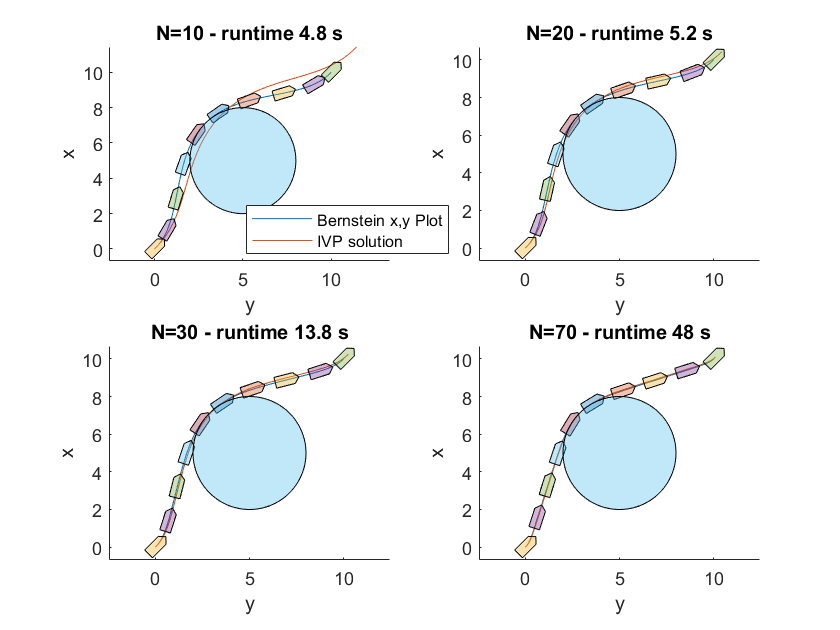
\includegraphics[width=0.8\textwidth]{Images/results/progressiveNexamples.png}
\caption{Results of Interatively increasing order}
\label{fig:progressiveNexamples}
\end{figure}



\par We can see how to cost varies with increase of order $N$ and how the solution of the \ac{IVP} becomes closer and closer to the plot of $xy$.





\section{Multiple Vehicles}

\par In figure \ref{fig:multiplevehicles} we can see how computation time quickly grows with even a small number of vehicles for a Medusa model and using the sampling approach for deconfliction discussed in \ref{sec:mindistintveh}.

\begin{figure}[h!]
\centering
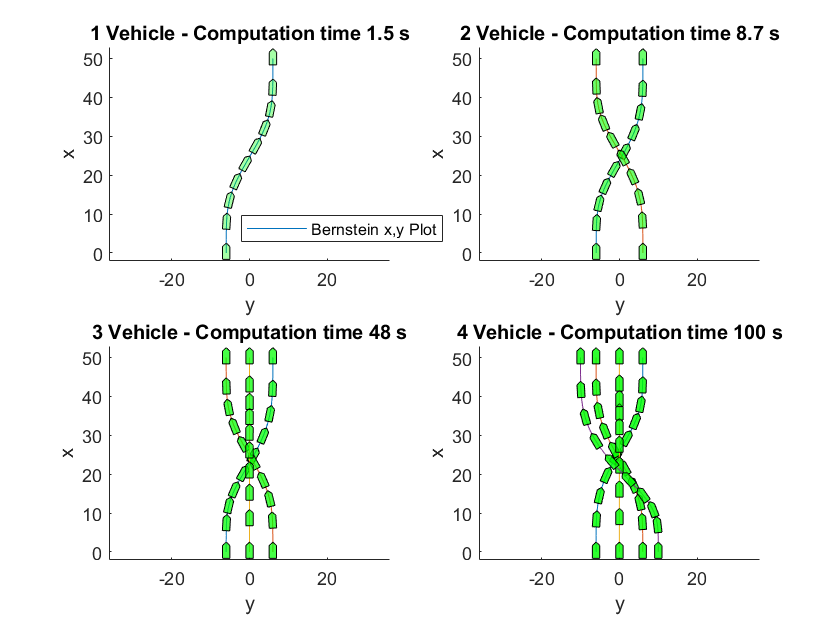
\includegraphics[width=0.8\textwidth]{Images/results/multiplevehicles.png}
\caption{Solutions of order $N=10$ with multiple vehicles}
\label{fig:multiplevehicles}
\end{figure}


\par And at last an example with 3 vehicles and 1 obstacle, in figure \ref{fig:finalexample}

\begin{figure}[h!]
\centering
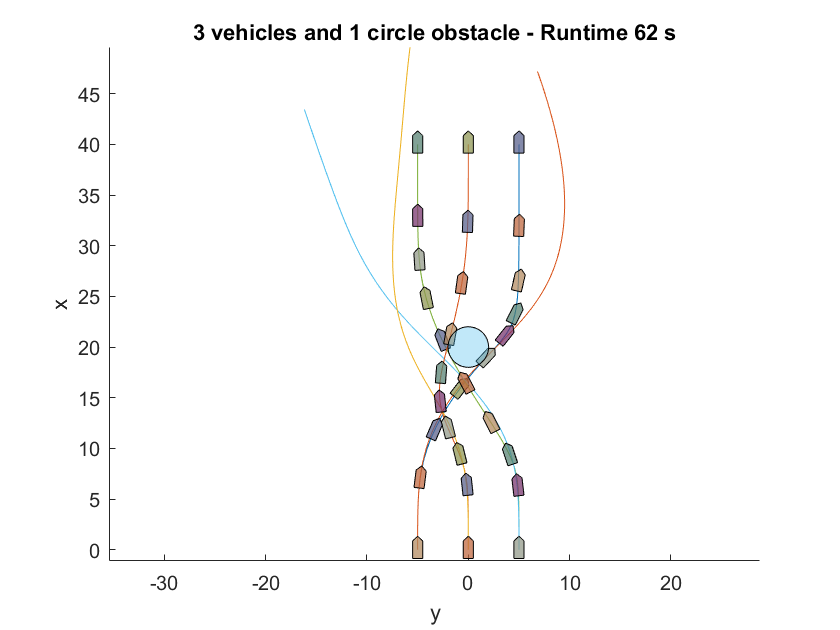
\includegraphics[width=0.8\textwidth]{Images/results/finalexample.png}
\caption{Solution of order $N=10$ with 3 vehicles and 1 circle obstacle}
\label{fig:finalexample}
\end{figure}